%%%%%%%%%%%%%%%%%%%%%%%%%%%%%%%%%%%%%%%%%%%%%%%%%%%%%%%%%%%%%%%%%%%
%%% Documento LaTeX 																						%%%
%%%%%%%%%%%%%%%%%%%%%%%%%%%%%%%%%%%%%%%%%%%%%%%%%%%%%%%%%%%%%%%%%%%
% Título:		Capítulo 5
% Autor:  	Ignacio Moreno Doblas
% Fecha:  	2014-02-01, actualizado 2019-11-11
% Versión:	0.5.0
%%%%%%%%%%%%%%%%%%%%%%%%%%%%%%%%%%%%%%%%%%%%%%%%%%%%%%%%%%%%%%%%%%%
% !TEX root = A0.MiTFG.tex

\chapterbegin{Implementación}
\label{chp:App2}
\minitoc

En este capítulo se explicarán los bloques que forman parte de la implementación de
la codificación de la señal en la transmisión y del sistema de decisión y la 
decodificación en la recepción. Se mostrarán algunos esquemáticos equivalentes y 
sus respectivas simulaciones para comprobar su correcto funcionamiento.

\section{Sistema general}
En primer lugar, para tener una visión general alejada del bajo nivel se presenta la 
figura \ref{general}, que contiene los bloques que forman parte del proyecto. Los bloques sobre 
los que se ha trabajado en este proyecto son el transmisor (axi\_vlc\_transmitter) para
la codificación y el receptor (axi\_vlc\_receiver) para la decodificación además de añadir
al bloque del filtro adaptado (mf\_0) el sistema de decisión para pasarle al receptor
la mejor señal posible. Es importante destacar que el bloque correspondiente al reloj es 
fundamental para establecer la frecuencia del sistema y que el bloque correspondiente a la 
interconexión AXI también es imprescindible ya que, entre otras cosas, permite la 
comunicación con la memoria RAM para leer y/o escribir la trama de datos. Ambos bloques
están predefinidos en la plataforma Vivado.

\begin{figure}[ht]
    \centering
    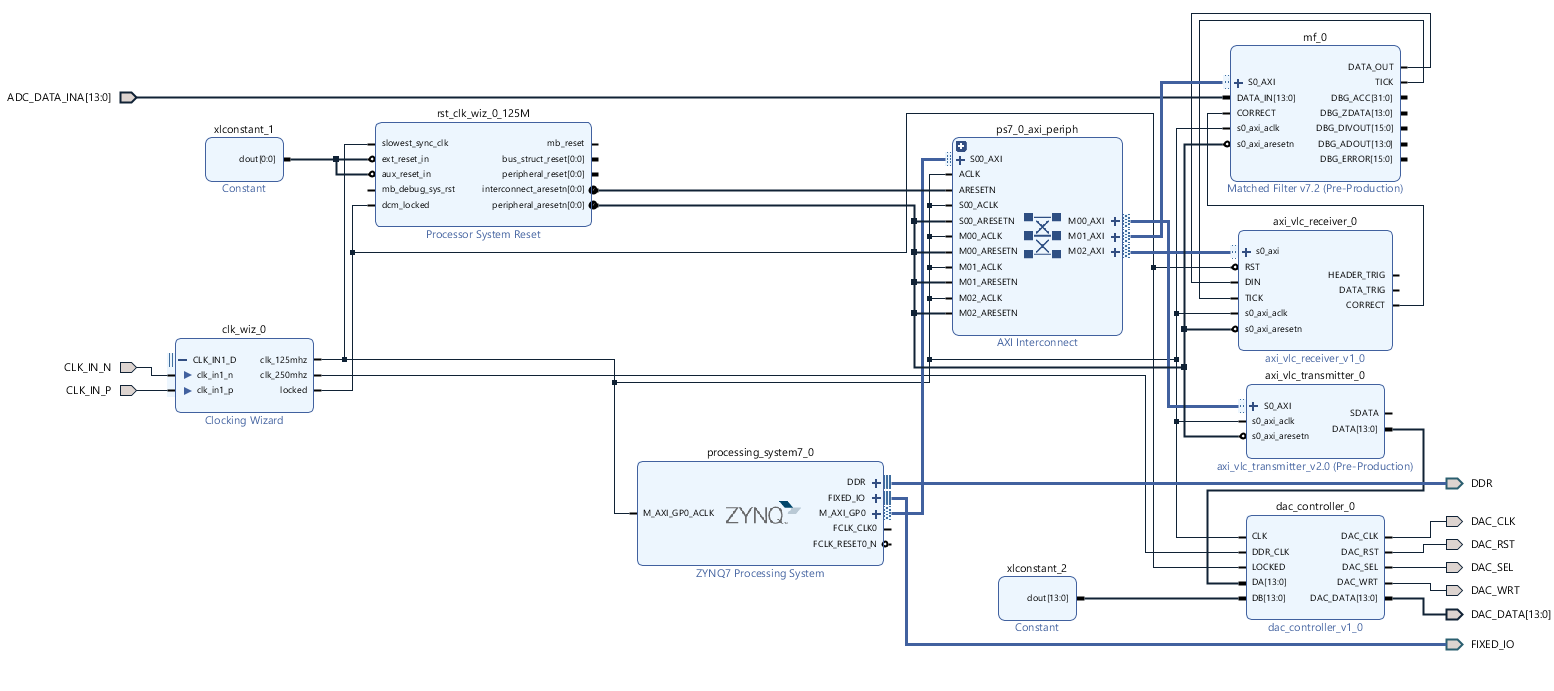
\includegraphics[scale=0.5]{./figuras/general.png}
    \caption{\small{Diagrama de bloques general del sistema completo.}}
    \label{general}%
\end{figure}

Como se aprecia en la figura, el sistema está formado por todos los bloques necesarios para 
la transmisión y recepción por lo que, con este diseño, la FPGA está programada para poder 
realizar cualquiera de las dos funciones en cualquier momento.

Aunque los tres bloques en los que se basa este trabajo
se desarrollarán en detalle en este capítulo, es importante tener una
perspectiva conjunta del sistema para tener claro
el flujo de funcionamiento. Para ello se presenta
la figura \ref{trans}, que muestra el diagrama de flujo de la transmisión
y la figura \ref{rec}, de la recepción para diferenciar los bloques que forman parte en cada 
proceso y entender la actividad global de cada parte del sistema. 

\begin{figure}[ht]
	\centering
	  \begin{minipage}{7cm}
		\centering
		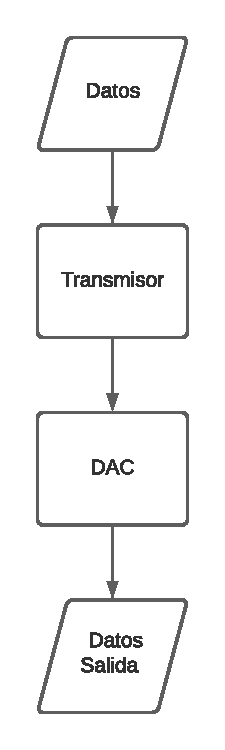
\includegraphics[scale=0.83]{./figuras/flujo_trans.pdf}
		\caption{\small{Diagrama de flujo de la transmisión de datos}}
		\label{trans}
	  \end{minipage}%
	  \hspace{5mm}
	  \begin{minipage}{7cm}
		\centering
		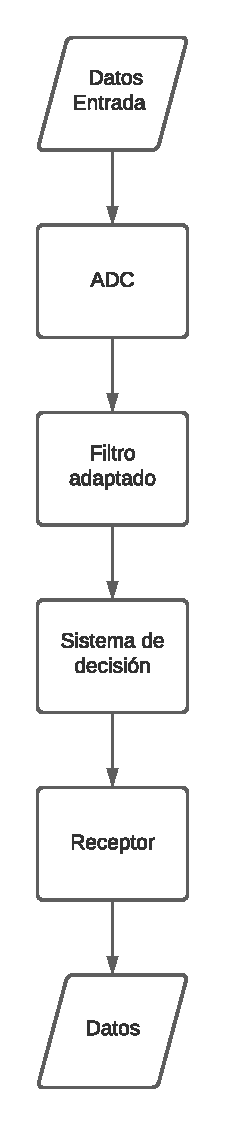
\includegraphics[scale=0.55]{./figuras/flujo_receptor.pdf}
		\caption{\small{Diagrama de flujo de la recepción de datos}}
		\label{rec}
	  \end{minipage}
\end{figure}

Antes de comenzar a desarrollar los bloques es importante destacar que cada paquete 
transmitido y recibido está formado por bits de sincronismo, bits de cabecera y la propia 
trama de datos. 

\newpage

\section{Transmisor}
% -Selector del esquema de codificación (sincronismo manchester y trama en la codificación elegida)
% -Diagramas de Markov para implementar la codificación
El primer bloque a desarrollar es el bloque transmisor. La función principal de este 
bloque es leer los datos de entrada y transmitirlos codificados no sin antes generar una 
dirección. Lo verdaderamente interesante en este bloque es como se ha implementado la 
codificación del esquema de señalización deseado.

En un primer momento se realizó la codificación del paquete entero, incluyendo los bits
de sincronismo, con el esquema de señalización empleado. Es decir, que toda la trama se 
codificaba de la misma manera. Sin embargo, tras varios estudios y pruebas se llegó a la 
conclusión de que, para alcanzar mayor velocidad de transmisión y mayor robustez, es más 
óptimo codificar la señal de sincronismo del paquete con codificación Manchester. Esto se 
debe a que es el único esquema de codificación que máxima la frecuencia de trabajo ya 
que la frecuencia de Manchester es siempre el doble de la frecuencia de dato. La 
ventaja que le proporciona al sistema está relacionado con el filtro adaptado y el 
algoritmo de Gardner. 

Aunque no compete explicar el funcionamiento detallado del filtro adaptado si es 
óptimo decir que su funcionamiento es vital para una mejor recuperación de la señal 
recibida por el canal de luz y que, a gran escala, se basa en muestrear en los picos
de la señal gracias al algoritmo de Gardner. Como es natural, la señal suele llegar 
distorsionada y es durante la trama de sincronismo donde el algoritmo de Gardner entra 
en efecto para calcular cuáles son los momentos óptimos de muestreo para una vez llegue 
la trama de datos estar bien colocado. 

De acuerdo con esto, cuanto mejor sea la trama de sincronismo mejor será el sistema, 
es decir, lo
óptimo es que haya los máximos picos posibles y eso se maximiza con el uso de la 
codificación Manchester.

Debido a este efecto, se cambió la estructura del transmisor para siempre transmitir la 
trama de sincronismo con la codificación Manchester y el resto del paquete con el esquema 
de codificación deseado.

Para reproducir este cambio de codificación en el proyecto se ha impementado un proceso 
dentro del módulo principal que consiste en empezar a codificar con Manchester, ya
que los primeros bits son sincronismo, y hacer una cuenta hasta que dicho valor 
coincida con el número de bits de sincronismo, que es un valor conocido. Esta cuenta
se realiza a partir de la dirección inicial del paquete y el valor final es la suma de 
dicha dirección inicial más el número de bits de sincronismo. Una vez se 
produce esto se cambia a codificar con el esquema de codificación deseado. Lo más 
crítico en este cambio es que los procesos de codificación deben estar perfectamente 
sincronizados para no perder ningún bit. Para entender mejor este funcionamiento se 
presenta la figura \ref{selec_code} 
que esquematiza a través de un diagrama la codificación con los dos esquemas y la
figura \ref{cuenta} que esquematiza la cuenta de sincronismo.

\begin{figure}[ht]
    \centering
    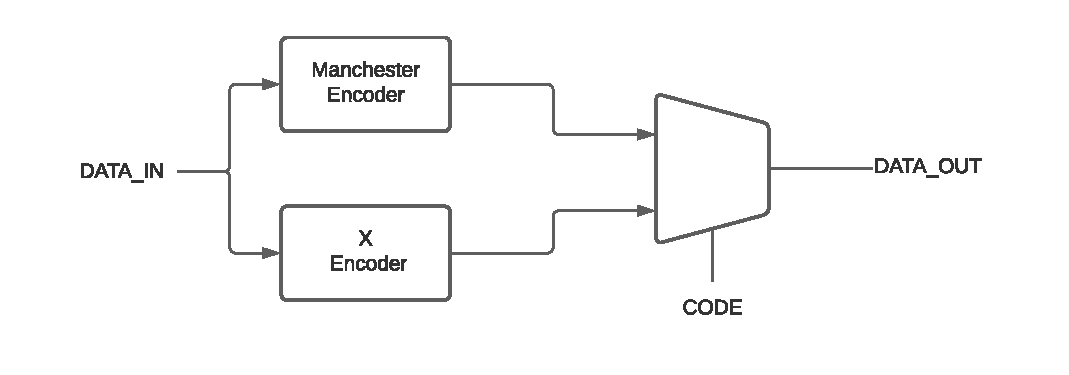
\includegraphics[scale=0.8]{./figuras/selec_code.pdf}
    \caption{\small{Selector de codificación.}}
    \label{selec_code}%
\end{figure}

\begin{figure}[ht]
    \centering
    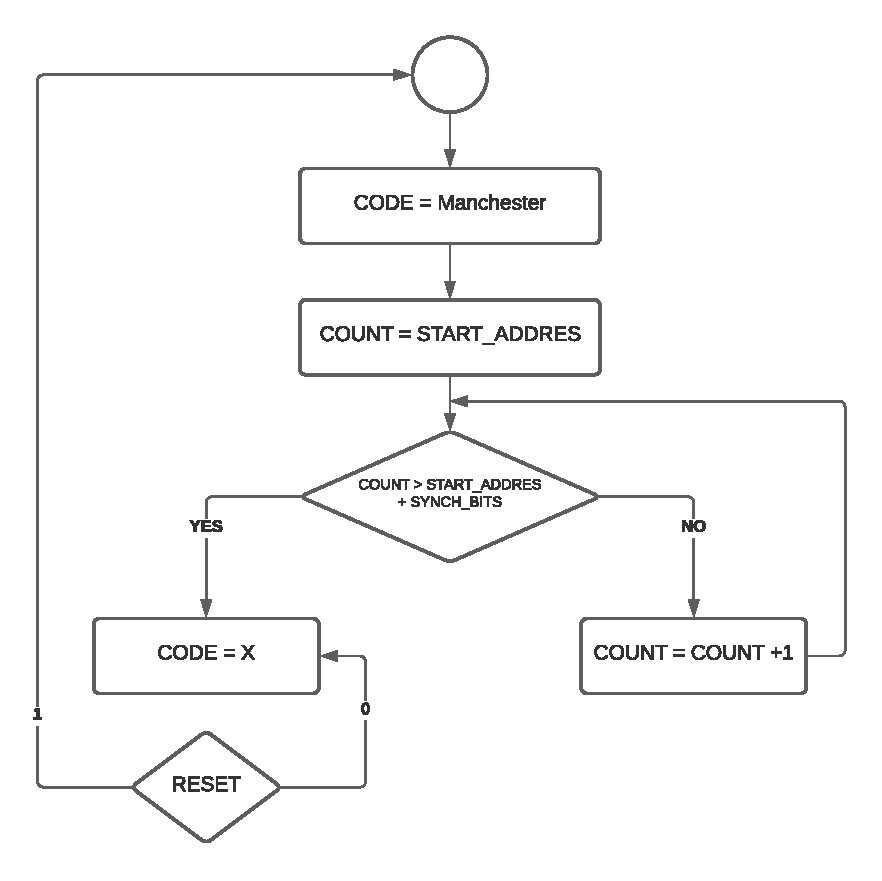
\includegraphics[scale=0.65]{./figuras/cuenta.pdf}
    \caption{\small{Cuenta de sincronismo.}}
    \label{cuenta}%
\end{figure}

Una vez explicado cómo el sistema cambia de codificación se continúa con la explicación 
de cómo se ha implementado la codificación del dato de entrada. El enfoque principal es 
la aplicación de máquinas de estados. Esto se debe a que es muy intuitivo traducir
los diagramas de trellis en diagramas de Markov o máquinas de estados. Lo que es 
crucial en la codificación es que hay que trabajar al doble de frecuencia de entrada
ya que un bit de entrada es codificado con dos de salida. 

Sin embargo, para codificar 4PPM no se puede codificar de esta manera ya que se 
codifican parejas de bits y no sigue ningún esquema de trellis. Esto implica mayor 
dificultad a la hora de implementarlo puesto que hay que leer de dos en dos teniendo
especial cuidado en no repetir datos de entrada y codificar de cuatro en cuatro. Para
esto hay que seguir trabajando al doble de frecuencia y codificar en función de la 
pareja leída tal y cómo se explicó en su apartado teórico.

La figura \ref{sim_tx_cancel} muestra una simulación de la codificación de la señal de entrada 
aplicando el esquema de codificación cancelación de pulsos. Hay que aclarar que 
la señal TICK va al doble de frecuencia de dato para poder codificar una pareja 
por cada bit de entrada. 

\begin{figure}[ht]
    \centering
    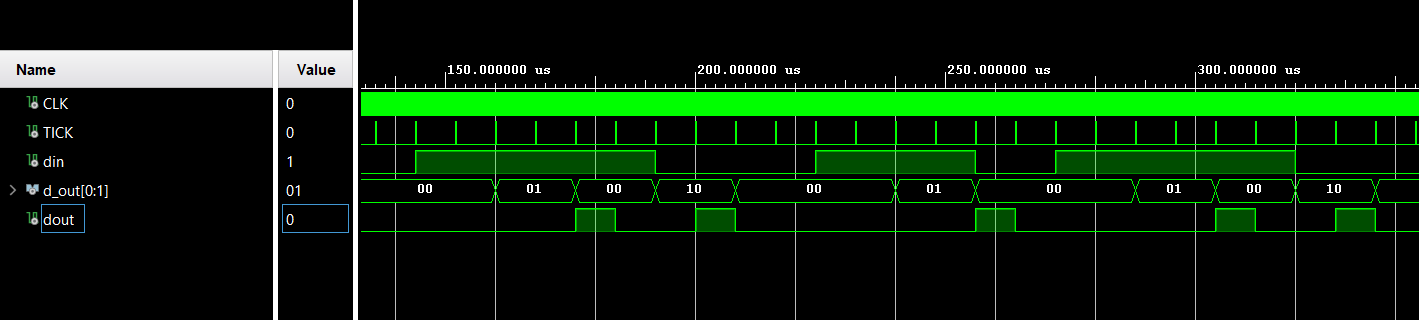
\includegraphics[scale=0.35]{./figuras/sim_cod_cancel.png}
    \caption{\small{Simulación del transmisor con cancelación de pulsos.}}
    \label{sim_tx_cancel}%
\end{figure}

\section{Receptor}
El segundo bloque es el receptor. La función principal de este bloque es desglosar el 
paquete para identificar cada parte del mismo y sobre todo decodificar la trama.

Hay que destacar que el paquete está formado por una trama de sincronismo, de cabecera
y de datos. El receptor empieza en modo sincronismo, es decir, espera a recibir 
la mitad de los bits de sincronismo totales, momento en el que avisa al módulo del 
filtro adaptado que ya está sincronizado y pasa a esperar a recibir el patrón del 
paquete. Cabe recalcar que los bits de sincronismo vienen en Manchester y lo demás
con la codificación elegida. Es importante saber que los bits de sincronismo y de 
patrón no se decodifican ya que hacerlo no tendría ningún impacto en la recepción.

Una vez se recibe correctamente el patrón se recibe la cabecera y se realiza el 
cálculo CRC para comprobar que el paquete es correcto y continuar con la recepción o 
desechar el paquete en caso contrario.

Tras lo comentado anteriormente se implementa la decodificación de la trama de datos
que es lo que se recibe a continuación. A la hora de implementar la decodificación
también hay diferencias entre pulsos alternos y cancelación de pulsos respecto a 4PPM. 

Para pulsos alternos y cancelación de pulsos se decodifica trabajando con parejas de 
bits, ya que cada pareja corresponde a un dato. Por lo tanto, es fundamental elegir las 
parejas adecuadas para lo que se utilizan registros para guardar el primer de bit de la 
pareja y no decodificar hasta que no se recibe el segundo y así sucesivamente. Esta 
decodificación se realiza implementando una máquina de estado inversa, es decir, se ha 
creado una máquina de estados correspondiente a la decodificación que, como es lógico, 
guarda relación con la correspondiente a la codificación pero no es igual.

Para 4PPM se decodifica trabajando con cuartetos de bits ya que sabemos que en este 
esquema se codifican parejas de datos. Lo más importante en este esquema es elegir
bien los cuartetos adecuados sin mezclarlos ya que su decodificación se basa en 
comprobar con cuál de los cuatro cuartetos posibles coincide el cuarteto recibido para 
traducirlo a su respectiva pareja de datos.

Una vez se decodifican los datos, estos se escriben en la memoria RAM del sistema para 
su posterior lectura en el programa en C.

% La figura x muestra una simulación de la decodificación de la señal aplicando el 
% esquema x. 

% [FOTO DECODIFICACIÓN del esquema que quiera]

\section{Sistema de decisión}
		% -Hard-decoding (umbral en la mitad)
		% -Soft-decoding (cómo se implementa el cálculo de la distancia euclídea)
		% -Algoritmo de Viterbi (que efecto tiene y cómo se implementa la mirada al pasado para descartar opciones que tienen probabilidad 0)

La implementación de los sistemas de decisión es crucial para la mejora en el 
funcionamiento del sistema en recepción. Por lo tanto, se va a desarrollar la 
implementación de cada uno de los tres sistemas de decisión.

\subsection{Hard-decoding}
La implementación de \textit{hard-decoding} es la más sencilla y rápida de todas ya que 
sólo hay que colocar un umbral en la mitad del rango del ADC. Aquí es imprescindible
destacar que la resolución del ADC es de 14 bits por lo que su rango es de 0 a 
16384 siendo 0 equivalente a +1V y 16384 equivalente a -1V. Sin embargo, en el filtro 
adaptado se realiza un mapeo de la señal para que su interpretación sea más intuitiva. 
Este mapeo hace que la señal digital tenga 'signo', lo que provoca que la señal cambie su 
rango de valores y sea una señal simétrica siendo su rango [-8192,8191] en el que 
-8192 equivale a -1V ('0') y 8191 a +1V ('1'). 

Una vez conocido este mapeo la colocación del umbral se implementa mirando el bit más 
significativo de la muestra ya que si este bit es '1' significa que la señal es 
negativa por lo que se traduce como un '0' lógico y si el bit más significativo es un 
'0' implica que la señal es positiva por lo que sería un '1' lógico.

De esta manera se coloca el umbral en la mitad de la señal siendo muy sensible a 
errores provocados principalmente por la inclusión de corriente continua que provoca
que la señal no esté centrada.

Además, es fundamental explicar que en nuestro caso para los tres esquemas de 
codificación empleados el umbral no se colocaría en 0. Esto se produce porque al 
ser esquemas no equiprobables el efecto que provoca el receptor óptico es que la 
señal no se simetrice perfectamente por lo que la señal tiene un efecto en la que está
'subida' y no se encuentra en el rango [-8192,8191] si no que el valor negativo es más
elevado. Por este motivo, el umbral varía entre cada esquema según los cálculos 
realizados en el apartado teórico.

La figura \ref{sim_hard_4ppm} muestra una simulación del funcionamiento del sistema 
\textit{hard-decoding} para el esquema de codificación 4PPM. En ella se observa como 
este sistema depende de si la señal está por encima del umbral o no para determinar su 
valor sin tener en cuenta la naturaleza de la codificación. Por lo que no es capaz de 
corregir ningún error tal y como se aprecia en la imagen en el caso de '0011'. Una 
señal importante en la imagen es 'control' que es la que indica que ya se ha recibido la 
primera pareja del patrón y es el momento de trabajar con cuartetos.

\begin{figure}[ht]
    \centering
    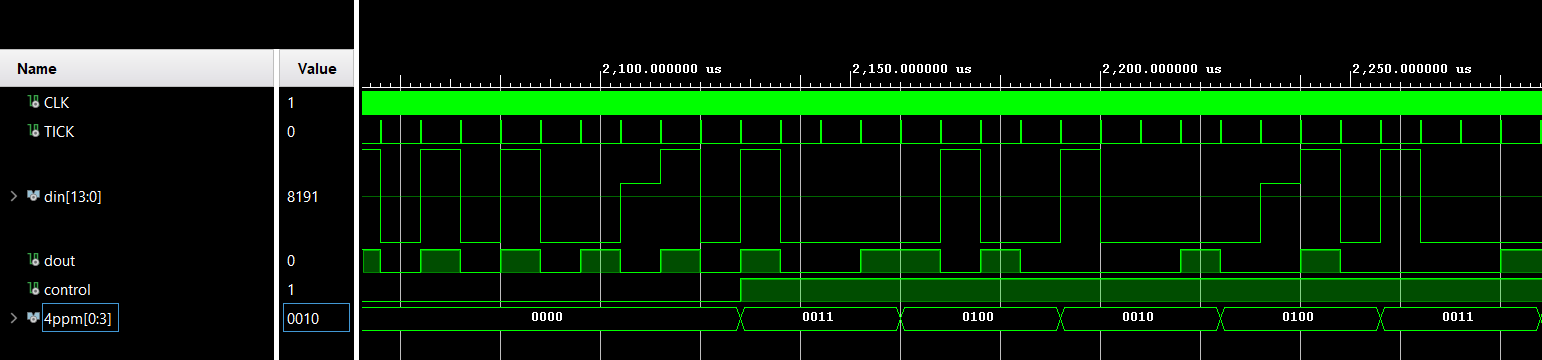
\includegraphics[scale=0.4]{./figuras/sim_hard_4ppm.png}
    \caption{\small{Simulación \textit{hard-decoding} con 4PPM.}}
    \label{sim_hard_4ppm}%
\end{figure}

\subsection{Soft-decoding}
La implementación de este sistema es más compleja que la anterior y por consecuencia
sus prestaciones son mejores.

Tal y como se comentó en el apartado teórico es imprescindible conocer las opciones 
posibles que se pueden dar en recepción con cada esquema de codificación empleado ya que
este método calcula a través de la distancia euclídea a que opción se parece más la 
que se ha recibido. Tanto para pulsos alternos como para cancelación de pulsos se 
trabaja con parejas de bits y para 4PPM se trabaja con cuartetos de bits.

Hay que destacar que tal y como se ha comentado en transmisión la trama de sincronismo
se transmite con Manchester y el resto del paquete con otra codificación. Por lo tanto,
a la hora de aplicar este método hay que diferenciar los cálculos para cada uno por lo 
que es clave saber cuál hay que aplicar en cada momento.

La implementación de \textit{soft-decoding} tiene dos puntos fundamentales para su 
correcto funcionamiento que son la realización correcta del cálculo de la distancia
euclídea y la correcta sincronización para calcular dicha distancia con las parejas o
cuartetos adecuados de la codificación correspondiente.

Lo más determinante es que para la implementación de este método es que hay 
que diferenciar entre pulsos alternos y cancelación de 4PPM.

Para pulsos alternos y cancelación, primero,
se aplica el cálculo con las opciones de Manchester, ya que el sincronismo viene con esa 
codificación, y cuando ya se han recibido la mitad de los bits totales de sincronismo 
(porque si se esperan a todos es muy difícil puesto que es normal que algunos bits del
principio se pierdan) se aplica el cálculo con las opciones de pulsos alternos o 
cancelación. Esto es posible porque las opciones de pulsos alternos y cancelación 
('00','01','10') contienen a las dos opciones de Manchester por lo tanto no habría
ningún problema si todavía falta algún bit de sincronismo por llegar. \label{xx}

La implementación de la distancia euclídea para pulsos alternos y cancelación se 
realiza comparando las distancias obtenidas de la pareja recibida con cada una de 
las tres opciones posibles mediante la aplicación de la fórmula descrita en el 
apartado teórico. Como los tres esquemas son no equiprobables y siguiendo lo 
desarrollado en el apartado teórico el valor bajo no será el máximo si no que subirá 
por lo que el valor del vector esperado en la fórmula cambiará para cada esquema de 
codificación según los cálculos realizados en el apartado teórico.
La dificultad está en la aplicación de la fórmula, principalmente,
porque los datos recibidos son vectores de bits. En un primer intento se realizó un 
módulo para operar con los vectores, sin embargo, presentó muchos problemas en
su desarrollo, debido a desbordes de los vectores y la necesidad de implementar varios
procesos con operaciones simples, y en su resultado, debido a un retardo desmesurado
para cada operación que provocaba fallos de tiempo de set-up. 

Tras concluir que hacerlo
de esta manera no era eficiente se cambió la visión y se ha realizado a través de una 
librería propia con funciones propias. Estas funciones corresponden con cada proceso 
necesario para la implementación siendo estos la conversión del dato de entrada 
vectorial a entero, el cálculo de las tres distancias euclídeas, la comparativa entre
todas para encontrar la menor de todas y sacar la pareja elegida de forma serie y en 
valor lógico (binario). Este proceso se representa en la figura \ref{euclidea}.

\begin{figure}[ht]
    \centering
    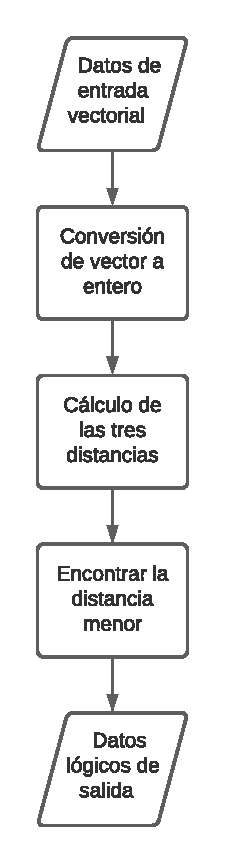
\includegraphics[scale=0.33]{./figuras/euclidea.pdf}
    \caption{\small{Diagrama de flujo.}}
    \label{euclidea}%
\end{figure}

Para 4PPM la dificultad reside en la sincronización ya que la implementación de la 
distancia euclídea es más sencilla. Esta implementación es más sencilla debido a que 
las cuatro distancias son máximas y representan diagonales entre sí. Esto implica que
no se necesite de la librería implementada si no que solo se comparen los cuatro bits
del cuarteto buscando el mayor que representará al único '1' del cuarteto. Esta 
comparación se realiza con los valores vectoriales recibidos para tener una mayor
precisión y eficacia en el cálculo.

La correcta sincronización si representa un reto mayor ya que hay que pasar de 
parejas a cuartetos. La primera parte es igual a la de pulsos alternos y cancelación
comentada con la diferencia de que el cambio entre parejas y cuartetos se produce
cuando se recibe '00' ya que no corresponde a código Manchester y sabemos a ciencia
cierta que es la primera pareja del patrón. Una vez se recibe esa pareja se trabaja
con los cuartetos.

La figura \ref{sim_4ppm} muestra una simulación del funcionamiento del sistema 
\textit{soft-decoding}
para el esquema de codificación 4PPM. En ella se ilustra como este sistema es capaz de 
regenerar la señal corrigiendo el error producido en el que un bit de la señal 
recibida es erróneo y cómo sale con valores lógicos y serializada. Aunque es 
díficil de entender a simple vista debido a los retrasos de los registros y las 
operaciones se ve su correcto funcionamiento.
Cabe destacar que este error no sería corregido en 
\textit{hard-decoding}.

\begin{figure}[ht]
    \centering
    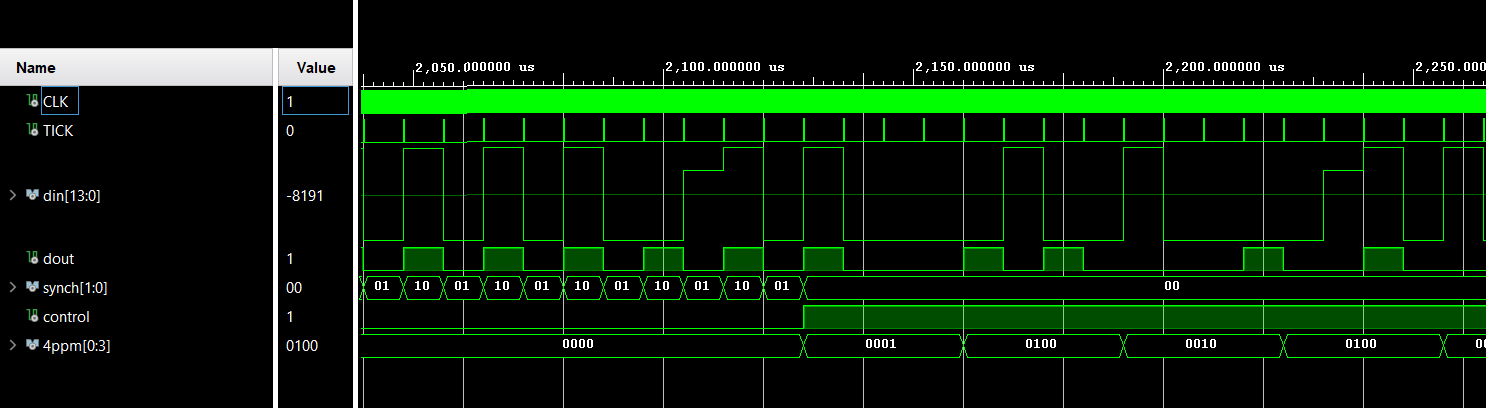
\includegraphics[scale=0.35]{./figuras/sim_4ppm.png}
    \caption{\small{Simulación \textit{soft-decoding} con 4PPM.}}
    \label{sim_4ppm}%
\end{figure}

\subsection{Algoritmo de Viterbi}
En este trabajo la implementación de Viterbi se basa en dotar de memoria al sistema 
para ampliar el rango de valores posibles para que el número de opciones descartadas
por la naturaleza de la codificación sea relevante. Hay que recordar que este 
sistema no se aplica a 4PPM ya que no se descarta ninguna opción cuando se le aplica
memoria. Para los otros dos esquemas si es óptimo. Al otorgarle memoria al sistema
ya no se trabaja con parejas de bits si no que se trabaja con cuartetos. Por lo tanto,
la sincronización se realiza de la misma manera que para 4PPM \textit{soft-decoding},
buscando la primera pareja de patrón, que es conocida, para en ese instante trabajar
con cuartetos de bits.

Para calcular las distancias euclídeas hay que ampliar la fórmula ya que ahora se 
trabaja con cuatro bits. Como es lógico se implementó siguiendo el proceso de la 
figura \ref{euclidea} con la única diferencia de que se realizan más comparaciones
y más cálculos lo que provoca que se ocupe más área de la FPGA y se tarde más 
tiempo, es decir, aumenta la complejidad del sistema. 

Tal y como se comentó en el apartado teórico este sistema es más eficaz para 
cancelación de pulsos ya que se descartan más opciones de las nueve posibles que 
en pulsos alternos, aunque para ambos la mejora respecto a no tener memoria (trabajar
con parejas y no cuartetos) es notable.

La figura \ref{sim_viterbi_cancel} 
muestra una simulación del funcionamiento del sistema para el esquema de
codificación cancelación de pulsos. En ella se observa la robustez del sistema ante 
errores de la señal recibida y cómo la memoria es clave para regenerar la señal de 
manera óptima.

\begin{figure}[ht]
    \centering
    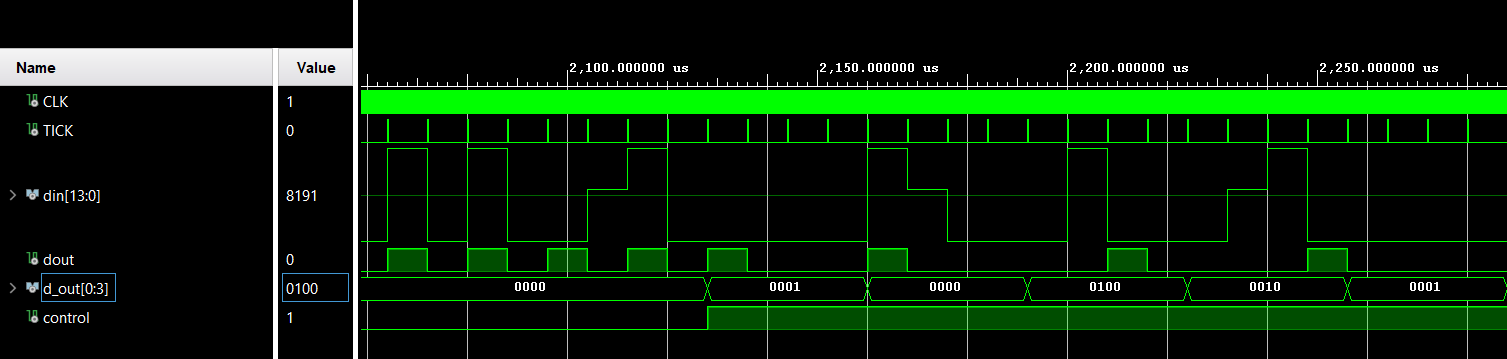
\includegraphics[scale=0.45]{./figuras/sim_viterbi_cancel.png}
    \caption{\small{Simulación algoritmo de Viterbi con cancelación de pulsos.}}
    \label{sim_viterbi_cancel}%
\end{figure}

\chapterend{}